\documentclass{article}[12pt]

% useful packages
\usepackage{fullpage}
\usepackage{amsmath,amssymb,amsthm,amsfonts}
\usepackage{graphicx}
\usepackage{enumerate}
\usepackage{algorithm,algorithmic}
\usepackage{xcolor}
\usepackage{bbm}
\usepackage{url}
\usepackage{caption,subcaption}

% theorem type environments
\newtheorem{thm}{Theorem}
\newtheorem{prop}{Proposition}
\newtheorem{lemma}{Lemma}
\newtheorem{cor}{Corollary}
\newtheorem{defn}{Definition}
\newtheorem{assump}{Assumption}
\newtheorem{example}{Example}
\newtheorem{conjecture}{Conjecture}

% frequently used symbols
\newcommand{\bE}{\mathbb{E}}
\newcommand{\bP}{\mathbb{P}}
\newcommand{\bQ}{\mathbb{Q}}
\newcommand{\bR}{\mathbb{R}}
\newcommand{\bS}{\mathbb{S}}
\newcommand{\bN}{\mathbb{N}}
\newcommand{\bZ}{\mathbb{Z}}
\newcommand{\sC}{{\mathcal C}} 
\newcommand{\sD}{{\mathcal D}} 
\newcommand{\sE}{{\mathcal E}} 
\newcommand{\sF}{{\mathcal F}} 
\newcommand{\sL}{{\mathcal L}} 
\newcommand{\sH}{{\mathcal H}} 
\newcommand{\sN}{{\mathcal N}} 
\newcommand{\sO}{{\mathcal O}} 
\newcommand{\sP}{{\mathcal P}} 
\newcommand{\sR}{{\mathcal R}} 
\newcommand{\sS}{{\mathcal S}}
\newcommand{\sU}{{\mathcal U}} 
\newcommand{\sX}{{\mathcal X}} 
\newcommand{\sY}{{\mathcal Y}} 
\newcommand{\sZ}{{\mathcal Z}}

% operators
\newcommand{\sign}{\mathop{\mathrm{sign}}}
\newcommand{\supp}{\mathop{\mathrm{supp}}} % support
\newcommand{\argmin}{\operatornamewithlimits{arg\ min}}
\newcommand{\argmax}{\operatornamewithlimits{arg\ max}}
\newcommand{\dist}{\operatorname{dist}}
\newcommand{\tr}{\text{tr}}
\newcommand{\vecop}{\text{vec}}
\newcommand{\st}{\operatorname{s.t.}}
\newcommand{\cut}{\setminus}
\newcommand{\ra}{\rightarrow}
\newcommand{\ind}[1]{\mathbbm{1}\left\{#1\right\}} 
\newcommand{\given}{\ | \ }

% grouping operators
\newcommand{\brac}[1]{\left[#1\right]}
\newcommand{\set}[1]{\left\{#1\right\}}
\newcommand{\abs}[1]{\left\lvert #1 \right\rvert}
\newcommand{\paren}[1]{\left(#1\right)}
\newcommand{\norm}[1]{\left\|#1\right\|}
\newcommand{\ip}[2]{\left\langle #1,#2 \right\rangle}

% code commands
\newcommand{\matlab}{\textsc{Matlab }}
\newcommand{\algname}[1]{\textnormal{\textsc{#1}}}

% header command
\newcommand{\homework}[4]{
    \pagestyle{myheadings}
    \thispagestyle{plain}
    \newpage
    \setcounter{page}{1}
    \setlength{\headsep}{10mm}
    \noindent
    \begin{center}
    \framebox{
        \vbox{\vspace{2mm}
            \hbox to 6.28in { {\bf STAT 672: Statistical Learning II
            \hfill Winter 2020} }
        \vspace{4mm}
        \hbox to 6.28in { {\Large \hfill Homework #1 \hfill} }
        \vspace{2mm}
        \hbox to 6.28in { \Large \hfill Due: #2 \hfill }
        \vspace{2mm}
        \hbox to 6.28in { {\it Student Name: #3} \hfill {\it Professor Name: #4}}
        \vspace{2mm}}
   }
   \end{center}
   \markboth{Homework #1}{Homework #1}
   \vspace*{4mm}
}

\begin{document}
\homework{2}{February 5th, 2020}{Ethan Lew}{Bruno Jedynak}

\section{Kernel approximation}
Kernel methods typically require to compute the kernel $(p,p)$ matrix 
\begin{equation}
K_{ij}=K(x_i,x_j)
\end{equation}
for $x_1,\ldots,x_p \in \mathcal{X}$. 
If $p$ is too large, say $p\geq 10^4$, this is prohibitive. Instead, one might want to find a low rank approximation. Here is one way to do it: 
\begin{enumerate}
\item choose $n < p$ elements $z_1,\ldots,z_n \in \mathcal{X}$, with $n$ not too large, say $n \leq 10^3$. One way is to choose them is at random.  
\item Notate as usual $H$ the RKHS with kernel $K$. 
\item Consider $V \subset H$, the subspace of $H$ spanned by the functions $K(.,z_i)$, for $1 \leq i \leq n$. 
\item Approximate for any $x,y \in \mathcal{X}$,
\begin{equation}
K(x,y) \sim \langle \pi_V(K(.,x),\pi_V(K(.,y) \rangle_H 
\end{equation}
where $\pi_V$ denote the orthogonal projection onto $V$. 
\end{enumerate}

Assume that $K_n$, the $(n,n)$ matrix with elements $[K_n]_{ij}=K(z_i,z_j)$ is positive definite. Notate $K(x,Z)=(K(x,z_1),\ldots,K(x,z_n))^T$. 
\begin{enumerate}
\item Show that 
\begin{equation}
\pi_V K(.,x) = \sum_{i=1}^n \alpha_i(x)K(.,x_i) \mbox{ with } \alpha_i(x)=K_n^{-1}K(x,Z)
\end{equation}
\item show that 
\begin{equation}
 \langle \pi_V(K(.,x),\pi_V(K(.,y) \rangle_H = K(x,Z)^T K_n^{-1} K(y,Z)
 \end{equation}
 
 Note that this method provides the approximation 
 \begin{equation}
K(x,y) \sim \phi(x)^T \phi(y) 
\end{equation}  
 where $\phi(.)=K_n^{-\frac{1}{2}}K(.,Z)$ is a vector in $\mathbb{R}^n$
\item Show that the RKHS over $\mathcal{X}$ with kernel $G(x,y)=\phi(x)^T\phi(y)$ is made of the functions $f_w(.)=w^T\phi(.)$, where $w \in \mathbb{R}^d$. 
 \end{enumerate}
 \section{Kernel K-means}
 
 In this exercise I walk you through the spectral algorithm for finding an approximate solution of kernel k-means. 
 
 Let $x_1,\ldots,x_n$ be $n$ points in a set $\mathcal{X}$. We have seen in class that the relaxation of the kernel k-means problem consists in solving 
 \begin{equation}
 \label{eq:kmeans}
 \max_{S,S^TS=I_k} \mbox{trace}\left(S^TKS\right)
 \end{equation}
 where $S$ is an $(n,k)$ matrix, with $n>k$ and $K$ is a psd matrix with at least $k$ non-zero e-values. 
 \begin{enumerate}
 \item Let us write $S=(S_1,\ldots,S_k)$, where $S_j$ are vectors of length $n$. 
 Verify that 
 \begin{equation}
 \mbox{trace}S^TKS = \sum_{j=1}^k S_j^T K S_j
 \end{equation}
 Consider now the problem 
 \begin{equation}
 \label{eq:2}
 \max_{S,S_j^TS_j=1,j=1\ldots k} \mbox{trace}\left(S^TKS\right)
 \end{equation}
 Using Lagrange multipliers $\lambda=(\lambda_1,\ldots,\lambda_k)^T$, solving this problem is equivalent to solving 
 \begin{equation}
 max_{S,\lambda} J(S,\lambda) 
 \end{equation}
 with 
 \begin{equation}
 J(S,\lambda) =  \sum_{j=1}^k S_j^T K S_j - \sum_{j=1}^k \lambda_j S_j^TS_j
 \end{equation}
 \item Compute the gradients with respect to $S_j$ of $J(S,\lambda)$ for $j=1\ldots k$ and show that these gradients vanish when $S_1,\ldots,S_k$ are e-vectors of $K$ with e-values $\lambda_1,\ldots,\lambda_k$.  
 \item Choose these e-vectors to be orthogonal and with norm 1. Compute then $J(S,\lambda)$ and show that $\lambda_1,\ldots,\lambda_K$ have to be chosen to be the largest $k$ eigenvalues of $K$. 
 \item Argue that you have solved (\ref{eq:kmeans}). 
 
 \item This provides a recipe for solving kernel k-means: 
 \begin{enumerate}
 \item compute $S=(S_1,\ldots,S_k)$, the matrix of the first $k$ e-vectors of the matrix $K$. This is equivalent to mapping each point $x_i$ to the vector of $\mathbb{R}^k$, 
 \begin{equation}
 \phi(x_i)=(S_{1i},\ldots,S_{ki})
 \end{equation}
 \item Solve the clustering problem using a classical clustering algorithm, that is k-means or the Estimation Maximization algorithm (E.M.) fpr the data $\phi(x_1),\ldots,\phi(x_n)$
 \end{enumerate}
 Apply this to the data in file \mbox{kkm1.csv} for $k=2$. Use a package of your choice for the clustering algorithm. Show figures similar to the ones in figure 1, obtained with the Gaussian kernel in figures 1 and 2.  
 \item Show some results with a different kernel;
\end{enumerate}  
\begin{figure}
	\centering 
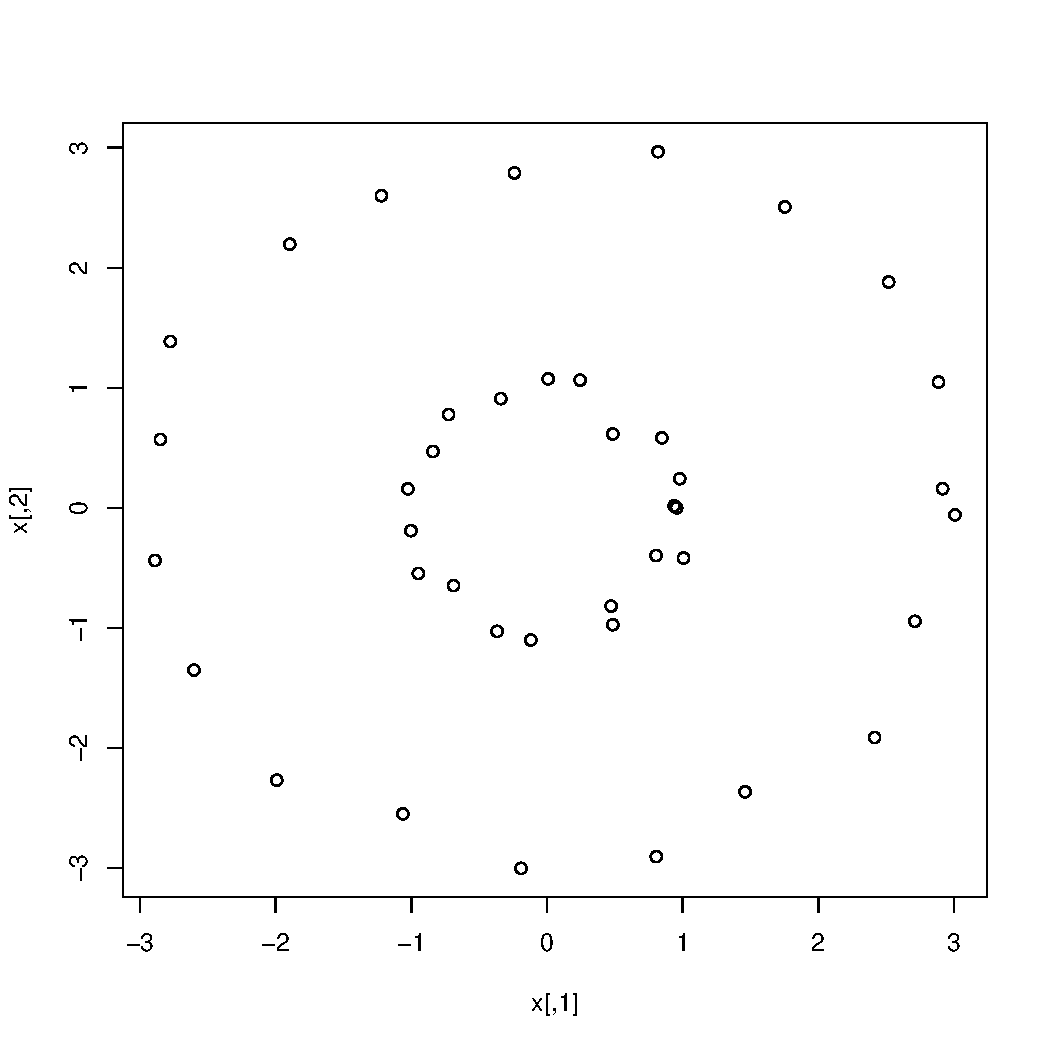
\includegraphics[width=0.3\textwidth]{img/data_for_kkm1.pdf}
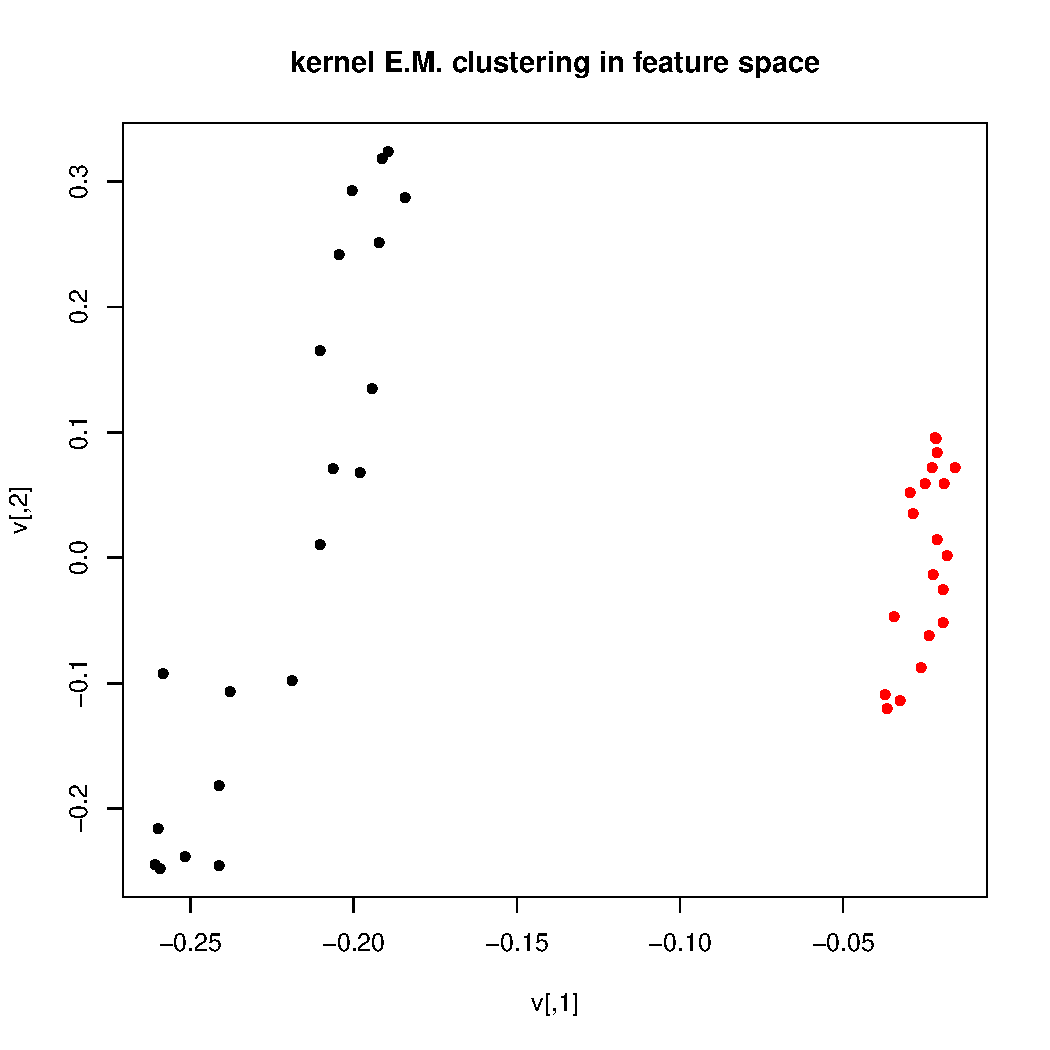
\includegraphics[width=0.3\textwidth]{img/kkmeans_feat.pdf}
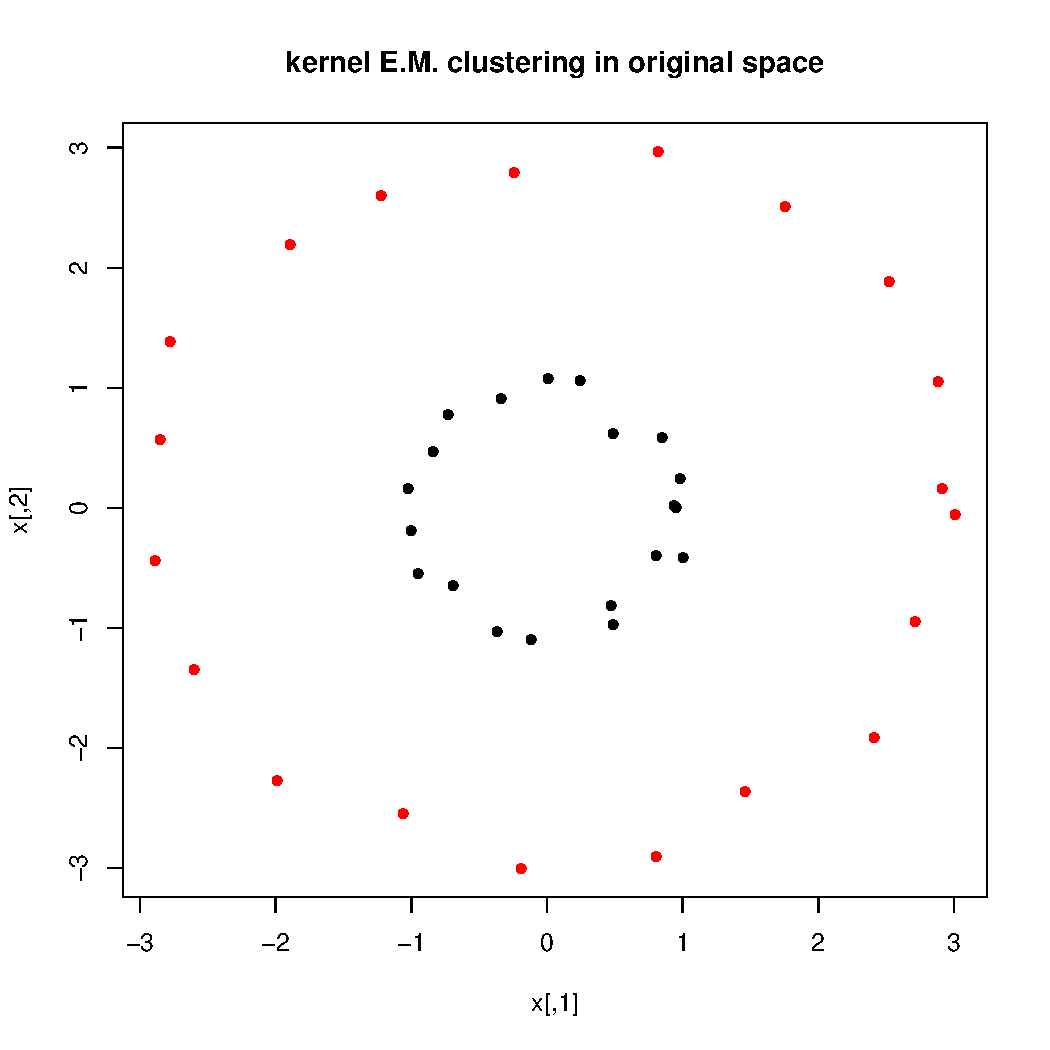
\includegraphics[width=0.3\textwidth]{img/kkmeans_orig.pdf}
\caption{Kernel k-means}
\end{figure}
\end{document}
